\documentclass[11pt,a4]{article} 
\usepackage[ansinew]{inputenc} %Schrifttyp und Umlaute
\usepackage{epsfig} %Nutzung von eps files
%\usepackage[dvips]{epsfig} %Nutzung von eps files
%\usepackage[final]{graphicx}    
%\usepackage[off]{auto-pst-pdf}     % necessary for psfrag to work
\usepackage{epstopdf} 

\usepackage[bf,sf,compact]{titlesec} 
\usepackage{fancyhdr} 
\usepackage{amsmath}
\usepackage{amssymb} %Symbole nach AMS
\usepackage{amstext}
\usepackage{theorem}
\usepackage{subfigure}
\usepackage{booktabs}

\usepackage{flafter}
\usepackage{exscale}
\usepackage{float}   % for minipages
\usepackage{psfrag}


\setlength{\parindent}{0cm} 
\setlength{\textwidth}{16cm}
\setlength{\oddsidemargin}{0cm}  
\setlength{\voffset}{-2,8cm}  
\setlength{\textheight}{25cm} 
\setlength{\arrayrulewidth}{0,3mm} 
\setlength{\textheight}{25cm} 

\renewcommand{\labelenumi}{\alph{enumi})} 
\sloppy



\begin{document} %hier geht es los

\thispagestyle{empty} 
\begin{tabular*}{16cm}{lr} \hline \\ %Tabelle mit zwei Spalten, in jeder Spalte eine minipage, neue Zeile mit \\
    \begin{minipage}{10cm} %Anfang minipage in linker Spalte, Breite 8cm
            \textsf{Technische Universit\"at Dortmund \\ %Schriftgröße smallface
            Department of Biochemical and Chemical Engineering \\
            Chair of Process Dynamics and Operations \\
            Prof.~Dr.~Sebastian Engell \\}
    \end{minipage} & %Ende minipage in linker Spalte
    \begin{minipage}{6cm} %Anfang minipage in rechter Spalte, Breite 8cm
            \setlength{\unitlength}{1cm} %Formatierung, Platzierung und Einfuegen des ASTLOGOS
            \begin{picture}(8,1) 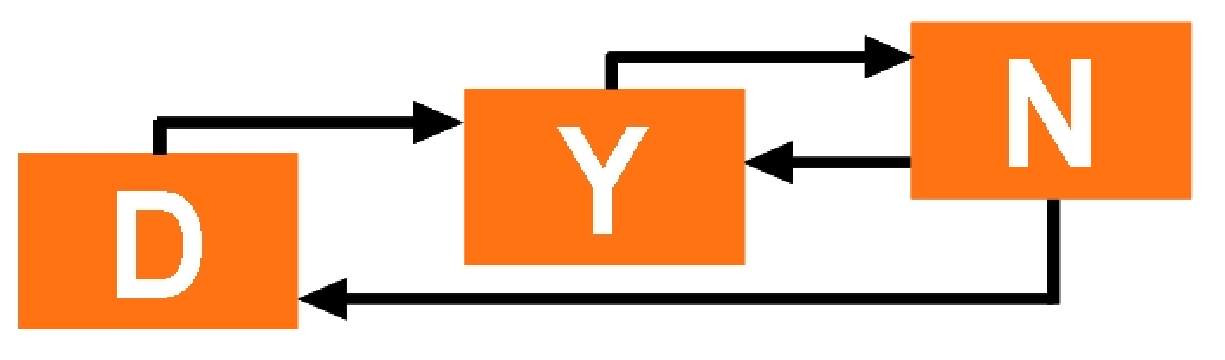
\epsfig{file= Astlogo.eps, width=5cm}
            \end{picture}\par
    \end{minipage} \\ \hline %Ende minipage in rechter Spalte
\end{tabular*} %Ende Tabelle




\vspace{5cm}

\begin{center} 

\LARGE{\bfseries EXAMPLE TITLE \\

    Automation \& Robotics 
    
    Group Project SS18 \\}
\end{center}



%%%%%%%%%%%%%%%%%%%%%%%%%%%%
\clearpage
\titleformat{\section}{\Large\bf}{\thesection:}{20pt}{}
\setcounter{enumi}{0} % !TeX encoding = UTF-8
\chapter*{\iftoggle{lang_eng}{Abstract}{Kurzfassung}}
Das ist die Kurzfassung. Hier sollte klar werden womit sich die Arbeit beschäftigt und die wichtigsten Aussagen sollen zusammengefasst werden. Richtwert is eine halbe Seite.

%%%%%%%%%%%%%%%%%%%%%%%%%%%%
\clearpage
\tableofcontents


\setlength{\textheight}{20cm}

\pagestyle{fancy} 
\lhead{Final report, TITLE, DD.MM.YYYY}
\chead{}
\rhead{Page \thepage}
\lfoot{}
\cfoot{}
\rfoot{} 
\renewcommand{\headrulewidth}{0.4pt} 

\setlength{\topmargin}{2cm} %oberer Rand bis Oberkante Kopfzeile

\makeatletter \def\usecounter#1{\@nmbrlisttrue\def\@listctr{#1}}
\makeatother 
\setcounter{figure}{0}
\setcounter{table}{0} 


%%%%%%%%%%%%%%%%%%%%%%%%%%%%
\titleformat{\section}{\Large\bf}{\thesection}{20pt}{}
\include{sections/introduction_marina}



%%%%%%%%%%%%%%%%%%%%%%%%%%%%
\clearpage
\titleformat{\section}{\Large\bf}{\thesection}{20pt}{}
\section{Theory} %

\begin{itemize}
\item Example
\item 
\end{itemize}



\label{LetzteSeite} %marker letzte Seite


\end{document}

\label{LetzteSeite} %marker letzte Seite
